\documentclass[11pt]{article}

\usepackage[T1]{fontenc}
\usepackage[utf8]{inputenc}
\usepackage{lmodern}
\usepackage[margin=1in]{geometry}
\usepackage{microtype}
\usepackage[numbers,sort&compress]{natbib}
\usepackage{booktabs}
\usepackage{tabularx}
\usepackage{array}
\usepackage{xcolor}
\usepackage{hyperref}
\usepackage{tikz}
\usetikzlibrary{arrows.meta,positioning,shapes.geometric}

\hypersetup{
  colorlinks=true,
  linkcolor=blue!50!black,
  citecolor=blue!50!black,
  urlcolor=blue!50!black
}

\newcolumntype{Y}{>{\raggedright\arraybackslash}X}
\newcommand{\signinum}{\texttt{signinum}}
\newcommand{\crate}[1]{\texttt{#1}}

\title{\signinum: WSI-shaped JPEG and JPEG 2000 codecs for digital pathology}
\author{
  Greg Furletti\\
  Independent researcher\\
  \texttt{https://github.com/jcwal1516/signinum}
}
\date{April 30, 2026}

\begin{document}

\maketitle

\begin{abstract}
Whole-slide imaging (WSI) systems in digital pathology rarely decode a single
image once. Viewers, quality-control tools, and analysis pipelines repeatedly
inspect and decode tiled JPEG, JPEG 2000, and high-throughput JPEG 2000
(HTJ2K) payloads while requesting small regions, reduced-resolution views, and
tile batches. General-purpose image decoders are mature, but their public APIs
usually expose whole-image operations rather than the caller-owned state,
region-of-interest, downscale, and device-output surfaces needed by WSI
readers. \signinum{} is an Apache-2.0 Rust codec workspace for these workloads.
It provides native JPEG and JPEG 2000 / HTJ2K inspection and decode APIs,
restart-marker and coded-unit metadata, row streaming, tile-batch decode,
Deflate/Zstd/LZW/Uncompressed tile decompression, and additive Metal and CUDA
adapter surfaces. The workspace deliberately excludes vendor slide-container
parsing so that readers can retain ownership of I/O, pyramid selection,
threading, cache policy, and viewport scheduling. This preprint describes the
software architecture, WSI-oriented API design, validation strategy, current
integration evidence, and limitations of the first public-source checkpoint.
\end{abstract}

\section{Introduction}

Digital pathology stores scanned tissue slides as very large, tiled,
multi-resolution images. Interactive and analytic workloads built on these
slides decode many small compressed payloads rather than one monolithic image:
a viewer pans across tissue, a quality-control tool samples fields of view, or
an analysis pipeline extracts regions at a requested magnification. These
operations put pressure on codec APIs. The caller often needs to inspect tile
metadata without full decode, request a source-coordinate rectangle, produce a
reduced-resolution output, reuse scratch allocation across thousands of tiles,
or hand decoded output directly to a GPU pipeline.

\signinum{} is a Rust workspace that implements codec primitives for those WSI
access patterns. It is not a slide reader and does not parse SVS, NDPI, DICOM
WSI, Mirax, Zeiss, Leica, Ventana, Philips TIFF, or other vendor containers.
Instead, a reader resolves compressed tile bytes and passes those bytes to
\signinum{} for inspection, CPU decode, tile decompression, or backend-tagged
surface production. This boundary is intentional: WSI readers differ in their
I/O model, pyramid policy, cache eviction, prefetch behavior, and viewer
integration, while codecs can provide a smaller and more reusable contract.

The first public-source checkpoint of \signinum{} is version 0.1.0. Its primary
supported surface is CPU-first WSI decode on native \texttt{x86\_64} and
\texttt{aarch64} hosts. Apple Metal adapters are validated on Apple Silicon
macOS. CUDA-named crates expose the same device-output API shape but are
fallback-only compatibility adapters in this checkpoint; they do not make a
runtime CUDA execution or NVIDIA performance claim.

\section{Statement of Need}

OpenSlide established a widely used vendor-neutral WSI reading foundation for
pathology software \citep{goode2013openslide}. However, OpenSlide is a
reader-oriented C library, not a collection of Rust codec components. A Rust
reader, viewer, or benchmarking harness may need reusable codec pieces while
retaining independent ownership of tile scheduling, memory reuse, concurrency,
and data movement.

General-purpose JPEG decoders such as libjpeg-turbo, \crate{zune-jpeg}, and
\crate{jpeg-decoder} remain important comparators and, in many settings, the
right tools \citep{libjpegturbo,zunejpeg,jpegdecoder}. Their public APIs are
not primarily shaped around WSI-specific tile streams, restart-marker
inspection, caller-owned scratch buffers, and source-coordinate ROI plus
reduced-resolution decode. JPEG 2000 and HTJ2K add further integration
constraints. OpenJPEG, Grok, OpenHTJ2K, and Kakadu cover important parts of
the JPEG 2000 ecosystem \citep{openjpeg,grok,openhtj2k,kakadu}, while the
licensing, runtime, language, or API assumptions of those projects may not
match a permissively licensed Rust WSI stack.

\signinum{} fills this gap by exposing WSI-oriented codec APIs under the
Apache-2.0 license. It is designed as a lower-level dependency for slide
readers and systems experiments rather than a replacement for existing slide
readers or every general-purpose codec deployment.

\section{Related Work}

WSI standards and practice combine image-codec work with vendor-container and
clinical-workflow concerns. DICOM WSI standardization gives one major
container model for pathology data \citep{dicomwsi}, while deployed scanners
continue to produce many TIFF-derived and proprietary layouts. OpenSlide
abstracts over several of those containers and has served as a compatibility
oracle for many pathology applications \citep{goode2013openslide}.

At the codec layer, JPEG remains common for WSI tiles, while JPEG 2000 and
HTJ2K are used where wavelet coding, codestream structure, or throughput
constraints are attractive \citep{iso15444_15,taubman2019fbcot}. Existing
codec libraries optimize broad image-codec use cases. \signinum{} uses them as
comparators where possible but exposes an API aimed at slide-reader
composition: borrowed parse surfaces, explicit scratch/context reuse,
source-coordinate ROI, decode-time downscale, row streaming, tile batches, and
backend-tagged device surfaces.

\section{Design Goals}

\signinum{} is organized around five design goals.

\textbf{Separate codecs from slide containers.} Slide readers own vendor
parsing, levels, tile coordinates, I/O, cache policy, and prefetch. Codec crates
operate only on compressed tile bytes and explicit decode requests.

\textbf{Expose WSI-shaped operations directly.} The API includes inspect,
full decode, ROI decode, reduced-resolution decode, combined ROI plus
downscale, row streaming, tile-batch decode, and tile decompression.

\textbf{Keep runtime state caller-owned.} The caller controls output buffers,
scratch pools, and decoder contexts. This makes allocation, threading, and
batch behavior visible to the application instead of hiding them behind a
global runtime.

\textbf{Make device output additive.} CPU decode remains available without GPU
dependencies. Adapter crates provide Metal or CUDA-facing surfaces only when a
caller requests those backends and the platform supports them.

\textbf{Surface errors and limitations explicitly.} Unsupported formats,
invalid rectangles, too-small buffers, too-small strides, row-sink failures,
and unavailable explicit backends are returned as errors rather than silent
success.

\section{Workspace Architecture}

The workspace is layered around \crate{signinum-core}, which defines shared
pixel formats, backend requests, rectangles, row sinks, scratch/context
contracts, and decode traits. Codec crates implement those traits for JPEG,
JPEG 2000 / HTJ2K, and tile-compression primitives. Adapter crates add
platform-specific device surfaces without forcing GPU dependencies into the
CPU codecs. Figure~\ref{fig:architecture} summarizes this dependency shape.

\begin{figure}[t]
\centering
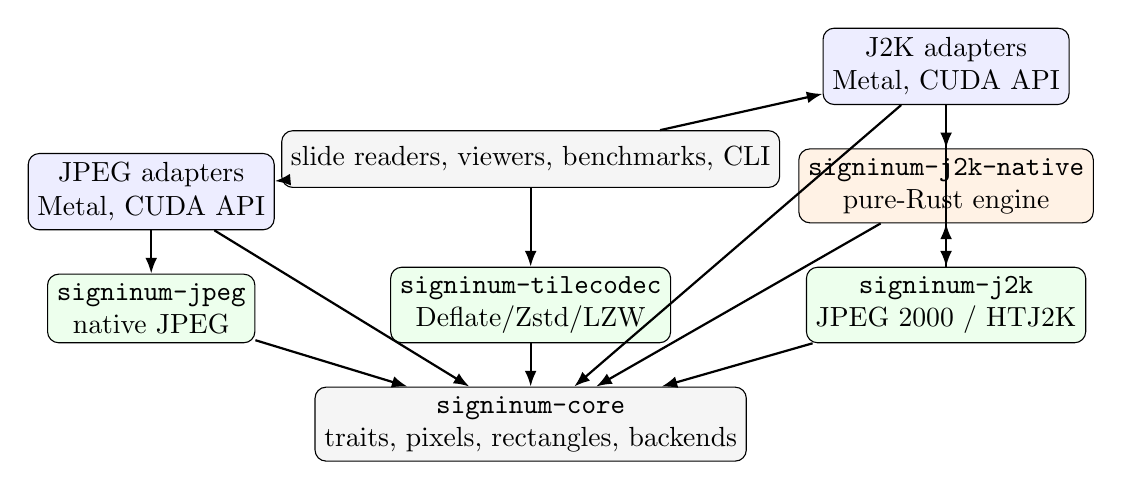
\begin{tikzpicture}[
  node distance=0.55cm and 0.75cm,
  layer/.style={draw, rounded corners, align=center, minimum width=3.1cm,
    minimum height=0.72cm, fill=gray!8},
  adapter/.style={draw, rounded corners, align=center, minimum width=2.6cm,
    minimum height=0.62cm, fill=blue!7},
  codec/.style={draw, rounded corners, align=center, minimum width=2.6cm,
    minimum height=0.62cm, fill=green!7},
  engine/.style={draw, rounded corners, align=center, minimum width=2.6cm,
    minimum height=0.62cm, fill=orange!10},
  arrow/.style={-{Latex[length=2mm]}, thick}
]
\node[layer] (core) {\crate{signinum-core}\\traits, pixels, rectangles, backends};
\node[codec, above left=of core] (jpeg) {\crate{signinum-jpeg}\\native JPEG};
\node[codec, above=of core] (tile) {\crate{signinum-tilecodec}\\Deflate/Zstd/LZW};
\node[codec, above right=of core] (j2k) {\crate{signinum-j2k}\\JPEG 2000 / HTJ2K};
\node[engine, above=of j2k] (native) {\crate{signinum-j2k-native}\\pure-Rust engine};
\node[adapter, above=of jpeg] (jpeggpu) {JPEG adapters\\Metal, CUDA API};
\node[adapter, above=of native] (j2kgpu) {J2K adapters\\Metal, CUDA API};
\node[layer, above=1.0cm of tile] (callers) {slide readers, viewers, benchmarks, CLI};

\draw[arrow] (jpeg) -- (core);
\draw[arrow] (tile) -- (core);
\draw[arrow] (j2k) -- (core);
\draw[arrow] (j2k) -- (native);
\draw[arrow] (native) -- (core);
\draw[arrow] (jpeggpu) -- (jpeg);
\draw[arrow] (jpeggpu) -- (core);
\draw[arrow] (j2kgpu) -- (j2k);
\draw[arrow] (j2kgpu) -- (native);
\draw[arrow] (j2kgpu) -- (core);
\draw[arrow] (callers) -- (jpeggpu);
\draw[arrow] (callers) -- (tile);
\draw[arrow] (callers) -- (j2kgpu);
\end{tikzpicture}
\caption{Workspace layering. Dependencies flow inward toward core traits and
types. GPU adapters are additive; removing them leaves the CPU codec stack
usable.}
\label{fig:architecture}
\end{figure}

\begin{table}[t]
\centering
\caption{Workspace responsibilities in version 0.1.0.}
\label{tab:crates}
\begin{tabularx}{\linewidth}{@{}lY@{}}
\toprule
Crate & Responsibility \\
\midrule
\crate{signinum-core} & Shared traits, pixel/sample types, backend requests,
device-surface contracts, rectangles, row sinks, and scratch/context types. \\
\crate{signinum-jpeg} & CPU-first JPEG inspect and decode, including WSI ROI,
scaled, row-streaming, and tile-batch surfaces. \\
\crate{signinum-j2k} & Public JPEG 2000 / HTJ2K inspect and decode wrapper over
the in-repo native engine. \\
\crate{signinum-j2k-native} & Internal pure-Rust JPEG 2000 / HTJ2K engine kept
under \texttt{\#![forbid(unsafe\_code)]}. \\
\crate{signinum-tilecodec} & Deflate, Zstd, LZW, and Uncompressed tile
decompression through the shared tile-decompress trait. \\
\crate{signinum-jpeg-metal}, \crate{signinum-j2k-metal} & Apple Metal
device-output adapters validated on Apple Silicon macOS. \\
\crate{signinum-jpeg-cuda}, \crate{signinum-j2k-cuda} & CUDA-facing API
compatibility adapters; explicit CUDA requests report unavailable in 0.1.0. \\
\crate{signinum-cli} & Host-neutral inspection entry point. \\
\bottomrule
\end{tabularx}
\end{table}

The API design is intentionally narrow. A reader passes compressed tile bytes
to a codec and provides output storage or a requested backend. It can keep a
\texttt{ScratchPool} and \texttt{DecoderContext} across a tile stream so hot
paths do not repeatedly allocate or rebuild codec tables. ROI coordinates are
expressed in source-image pixels. For combined ROI plus downscale, the returned
decoded rectangle is the scaled-grid coverage of the requested source
rectangle. Figure~\ref{fig:workflow} shows the common decode flow.

\begin{figure}[t]
\centering
\begin{tikzpicture}[
  node distance=0.8cm,
  step/.style={draw, rounded corners, align=center, minimum width=2.7cm,
    minimum height=0.72cm, fill=gray!8},
  path/.style={draw, rounded corners, align=center, minimum width=2.7cm,
    minimum height=0.72cm, fill=green!7},
  out/.style={draw, rounded corners, align=center, minimum width=2.7cm,
    minimum height=0.72cm, fill=blue!7},
  arrow/.style={-{Latex[length=2mm]}, thick}
]
\node[step] (bytes) {compressed\\tile bytes};
\node[step, right=of bytes] (inspect) {inspect / parse\\metadata only};
\node[path, right=of inspect] (request) {decode request\\full, ROI, scaled, batch};
\node[out, above right=0.65cm and 0.95cm of request] (cpu) {caller buffer\\CPU pixels};
\node[out, below right=0.65cm and 0.95cm of request] (device) {backend surface\\CPU, Metal, CUDA API};
\node[step, below=0.65cm of request] (state) {caller-owned\\scratch + context};

\draw[arrow] (bytes) -- (inspect);
\draw[arrow] (inspect) -- (request);
\draw[arrow] (request) -- (cpu);
\draw[arrow] (request) -- (device);
\draw[arrow] (state) -- (request);
\end{tikzpicture}
\caption{WSI decode workflow. The reader owns container parsing, I/O, cache
policy, and tile scheduling; \signinum{} owns codec inspection and decode of the
provided byte stream.}
\label{fig:workflow}
\end{figure}

\section{Validation Strategy}

\signinum{} validates behavior close to the codec boundary. Parser and decode
tests cover API behavior such as inspect, ROI, scaled output, combined ROI plus
scaled output, row streaming, tile batches, backend fallback, and error
surfaces. Comparator paths exercise libjpeg-turbo, OpenJPEG, and Grok where
those local dependencies are available. Fuzz targets exist for JPEG parse and
decode paths and tile decompression. Benchmark targets are compiled in CI so
performance harness drift is caught even when optional native comparator
libraries or GPU devices are not present.

As of April 29, 2026, the repository's \texttt{cargo test --workspace
--all-targets} run passed across the CLI, core, JPEG, JPEG Metal, JPEG CUDA,
JPEG 2000, JPEG 2000 Metal, JPEG 2000 CUDA, and tilecodec crates, including
benchmark smoke targets. That run included 165 \crate{signinum-jpeg} unit tests,
36 JPEG Metal tests, 75 native JPEG 2000 / HTJ2K tests, 43 JPEG 2000 Metal
tests, 10 tilecodec decompression tests, and focused parity/regression tests
against comparator paths where available. The JPEG corpus report over the
committed conformance fixtures completed 11 rows with zero failures. These
small fixtures are correctness smoke tests and are not used as WSI-scale
performance evidence.

\begin{table}[t]
\centering
\caption{Validation surfaces and claim boundaries.}
\label{tab:validation}
\begin{tabularx}{\linewidth}{@{}lY@{}}
\toprule
Surface & Current use \\
\midrule
Unit and integration tests & Exercise public decode, ROI, scaled, row,
tile-batch, adapter fallback, and error behavior. \\
Comparator tests & Compare selected JPEG and JPEG 2000 paths against
libjpeg-turbo, OpenJPEG, or Grok when those libraries are available. \\
Conformance fixtures & Provide committed byte-level smoke coverage with
manifested inputs and expected outputs. \\
Fuzz targets & Compile fuzz harnesses for JPEG parse/decode and tile
decompression paths. \\
Benchmark compile checks & Keep Criterion benchmark targets buildable in CI
without requiring performance-capable hardware. \\
GPU validation & Manual self-hosted workflows validate Metal runtime behavior
on Apple Silicon; CUDA crates remain compatibility surfaces in 0.1.0. \\
\bottomrule
\end{tabularx}
\end{table}

The native JPEG 2000 engine is kept under \texttt{\#![forbid(unsafe\_code)]}.
Workspace \texttt{unsafe} is isolated to CPU feature detection and audited JPEG
hot paths such as SIMD and low-level entropy-buffer handling.

\section{Integration Evidence}

\signinum{} is integrated as the production codec layer for \crate{statumen}, a
Rust WSI reader used by SlideViewer \citep{wsirs}. That integration exercises
the API on real slide workloads: SVS, NDPI, DICOM WSI, Zeiss, Mirax,
Hamamatsu VMS, Leica, Ventana, and Philips TIFF readers resolve compressed
tile bytes and pass decode work to \signinum{}. The companion parity harness
compares reader output against compatibility oracles including OpenSlide,
while the \signinum{} benchmark harness compares codec tasks against
libjpeg-turbo, \crate{zune-jpeg}, \crate{jpeg-decoder}, OpenJPEG, and Grok.

The current integration release gate passes on eight real local slides: two
NDPI slides, four JPEG-compressed SVS slides, and two JPEG 2000 SVS slides
from 94 MB to 2.5 GB. Representative \signinum-backed reader medians include an
NDPI B4 2k-region extraction at 45.8 ms versus 53.1 ms for OpenSlide and a
2.5 GB metastatic melanoma SVS 2k-region extraction at 20.3 ms versus 56.7 ms.
These are private local whole-reader measurements. They are included as
integration evidence that the codec boundary supports real WSI workloads, not
as public reproducible codec benchmark claims.

\section{Limitations}

\signinum{} is pre-1.0 software. The CPU WSI decode APIs are the primary
supported surface; GPU adapter APIs are still being hardened. Metal runtime
validation currently targets Apple Silicon macOS. CUDA-named crates are
source-published as fallback-only API compatibility adapters and do not ship a
runtime CUDA decoder in version 0.1.0.

The workspace does not parse WSI containers, manage a slide cache, schedule
threads, or implement a viewer runtime. This makes \signinum{} easier to compose
inside different readers, but it means downstream projects must provide those
policies themselves. JPEG 2000 / HTJ2K ROI plus reduced-resolution performance
thresholds and broader multi-host GPU benchmark coverage remain active
stabilization work before a 1.0 release.

\section{Availability and Reproducibility}

\begin{table}[t]
\centering
\caption{Availability metadata for the preprint checkpoint.}
\label{tab:availability}
\begin{tabularx}{\linewidth}{@{}lY@{}}
\toprule
Item & Value \\
\midrule
Repository & \url{https://github.com/jcwal1516/signinum} \\
Version discussed & 0.1.0 public-source checkpoint \\
Programming language & Rust 2021, minimum supported Rust version 1.94 \\
Code license & Apache-2.0 \\
Preprint license & Creative Commons Attribution 4.0 International (CC BY 4.0) \\
Primary arXiv category & \texttt{cs.SE} \\
Documentation & Repository \texttt{README.md}, \texttt{docs/architecture.md},
\texttt{docs/wsi-decode-api.md}, \texttt{docs/bench.md}, and
\texttt{docs/parity.md} \\
\bottomrule
\end{tabularx}
\end{table}

The narrow repository verification commands for the claims in this paper are
\texttt{cargo xtask test}, \texttt{cargo xtask bench-build}, and
\texttt{cargo xtask typos}. Runtime GPU validation is separate from hosted CI
because hosted runners do not provide the required devices; the repository
documents the self-hosted Metal and CUDA validation labels and claim
boundaries.

\section{AI Usage Disclosure}

Generative AI assistance was used to draft and revise manuscript text and to
check it against software-paper and arXiv source-package requirements. The
software design, implementation, tests, benchmark claims, and final technical
accuracy remain the author's responsibility.

\section{Acknowledgments}

The author thanks the maintainers of OpenSlide, libjpeg-turbo, \crate{zune-jpeg},
\crate{jpeg-decoder}, OpenJPEG, Grok, OpenHTJ2K, and Kakadu for the software
and documentation that make codec interoperability and benchmarking possible.

\bibliographystyle{unsrtnat}
\bibliography{references}

\end{document}
